\documentclass[pdflatex,sn-basic,iicol]{sn-jnl}

\usepackage{graphicx}
\usepackage{amsmath,amssymb,amsfonts}
\usepackage{booktabs}
\usepackage{multirow}
\usepackage{url}
\usepackage{placeins}
\usepackage{tabularx}
\usepackage{xcolor}
\usepackage{flushend}

\geometry{a4paper, textwidth=185mm, textheight=274mm, top=11mm, bottom=12mm, left=12.5mm, right=12.5mm}
\setlength{\columnsep}{5.5mm}
\let\table\tableorg
\let\endtable\endtableorg
\renewenvironment{table}[1][t]{\begin{tableorg}[#1]\centering\footnotesize}{\end{tableorg}}

\setlength{\textfloatsep}{4pt plus 1pt minus 1pt}
\setlength{\floatsep}{4pt plus 1pt minus 1pt}
\setlength{\intextsep}{4pt plus 1pt minus 1pt}
\setlength{\dbltextfloatsep}{4pt plus 1pt minus 1pt}
\setlength{\dblfloatsep}{4pt plus 1pt minus 1pt}
\setlength{\abovecaptionskip}{2pt}
\setlength{\belowcaptionskip}{2pt}
\setlength{\abovedisplayskip}{3pt plus 1pt minus 1pt}
\setlength{\belowdisplayskip}{3pt plus 1pt minus 1pt}

\makeatletter
\AtBeginDocument{
  \setlength{\bibsep}{0pt}
  \def\bibfont{\fontsize{7.0pt}{8.1pt}\selectfont}
}
\makeatother

\makeatletter
\renewcommand{\@maketitle}{%
  \hsize\textwidth\parindent0pt
  \ifx\@title\empty\else
    {\Titlefont\@title\par}
  \fi
  \ifnum\aucount>0
    \global\punctcount\aucount
    \vskip8pt
    \artauthors\par
    {\vskip3pt\addressfont\auaddress\par
     \ifnum\emailcnt>0\relax
       \ifx\corrauthemail\@empty\else{\ifnum\aucount>1*\fi}
       \textbf{Corresponding author:} \corrauthemail\par\fi
     \fi
    }
  \fi
  \vskip6pt
  {\printabstract\par}
  {\printkeywords\par}
  \vskip10pt
}
\makeatother

\graphicspath{{figures/}}

\begin{document}

\title[TopoRadar-Net for Alpine Avalanche Debris Mapping in Sentinel-1 SAR]{Topographic Radar Geometry-Guided Cross-Attention for Alpine Avalanche Debris Mapping in Sentinel-1 SAR: Cross-System Generalization Across the Alps, Pamirs, and Arctic}

\author*[1]{\fnm{Akshay} \sur{Sharma}}\email{akssha74@gmail.com}
\author[1]{\fnm{Lalji} \sur{Prasad}}\email{lalji.research@gmail.com}

\affil*[1]{\orgdiv{Department of Computer Science and Engineering}, \orgname{SAGE University}, \orgaddress{\city{Indore}, \postcode{452020}, \state{Madhya Pradesh}, \country{India}}}

\abstract{
Rapid, all-weather mapping of snow avalanche debris across rugged mountain terrain is critical for alpine civil protection, emergency response, and search-and-rescue operations. Synthetic Aperture Radar (SAR) sensors such as Sentinel-1 provide cloud-penetrating day-and-night winter monitoring, but bitemporal change detection in steep terrain suffers from foreshortening, layover, and radar shadow. We propose \textbf{TopoRadar-Net}, coupling bitemporal Sentinel-1 C-band SAR with local radar-topographic geometry through: (1) an analytical characterization of shift-invariant linear-convolution limits under non-stationary terrain projection; (2) multi-scale Radar-Topographic Cross-Attention Blocks; (3) a heuristic slope-prior loss audited for positive-label conflict; and (4) calibrated component- and corridor-level operational proxies. On AvalCD (7 events, 4 mountain systems, 993 polygons), TopoRadar-Net reaches $63.79\% \pm 1.88\%$ pooled macro F1, compared with Attention U-Net ($63.41\%$), SiamUNet-conc ($63.13\%$), ResU-Net ($62.92\%$), and SiamUNet-diff ($54.87\%$). Across three seeds, only the margin over SiamUNet-diff is significant ($+8.92\%$, $p=0.021$); the Attention U-Net difference is $+0.38\%$ ($p=0.869$). Seed-42 backslope differences do not persist as stable three-seed effects (Troms{\o}: $-0.34\% \pm 6.28\%$; Pamir: $+1.20\% \pm 7.73\%$). In Pamir, the false-alarm footprint is $30.0\%$ lower than Attention U-Net ($72.9\text{ ha}$ nominal-grid equivalent; $55.6\text{ ha}$ affine physical difference). The slope-prior mask overlaps $18.47\%$ of training positives and lowers held-out positive recall inside that mask relative to No-GeoLoss. Validation-calibrated Pamir road-corridor alerts achieve $83.0\%$ precision and $62.5\%$ recall, but the single Troms{\o} road-intersecting avalanche is missed in all seeds. These results establish competitive pixel performance and explicit operational failure boundaries, not a component-isolated mechanism or deployment-ready system.

}

\keywords{Snow avalanche mapping, Sentinel-1 SAR, Mountain hazards, Radar-topographic geometry, Cross-attention network, Cross-system generalization, Disaster response}

\maketitle

\section{Introduction}
\label{sec:intro}

Snow avalanches represent one of the most destructive natural hazards in alpine and high-mountain environments worldwide, posing severe threats to human life, critical transportation corridors, hydropower infrastructure, and mountain settlements across major mountain systems such as the European Alps, the Pamirs, the Himalayas, and Arctic mountain belts \citep{buehler2019automated, eckerstorfer2017remote, eaws2022size, techel2018spatial}. Rapid, systematic, and regional-scale mapping of avalanche release zones and debris deposits is vital for emergency search-and-rescue operations, hazard index updating, and retrospective validation of numerical avalanche dynamics models \citep{tompkin2021backscatter, muller2021synthetic}. However, conventional ground-based observations and optical satellite platforms (e.g., Sentinel-2, Landsat-8/9, PlanetScope) are frequently incapacitated during major avalanche cycles due to persistent cloud cover, winter blizzards, and polar night in high-latitude mountain regimes \citep{eckerstorfer2019near, vickers2016method}.

Synthetic Aperture Radar (SAR), particularly spaceborne C-band radar operating on the European Space Agency's (ESA) Sentinel-1 constellation, provides an indispensable all-weather, day-and-night observation system with a regular 6- to 12-day repeat cycle \citep{eckerstorfer2017remote, small2011flattening}. When snow avalanches release, dense slab flow and turbulent powder snow transport heavy snow masses down mountain chutes, depositing rough, granulated debris mounds in runout fans. This mechanical deposition alters the snowpack surface from smooth, undisturbed snow into rough, blocky debris, markedly increasing surface and volume backscatter ($\Delta \sigma^0 = \sigma^0_{\text{post}} - \sigma^0_{\text{pre}} > 0$) in both cross-polarization (VH) and co-polarization (VV) channels \citep{tompkin2021backscatter}.

Despite these promising physical principles, automated SAR change detection in rugged alpine terrain has historically suffered from acute false alarm rates and severe geometric distortions \citep{bianchi2021snow, gatti2026avalanche}. In steep topography, the side-looking imaging geometry of SAR creates complex radiometric distortions:
\begin{enumerate}
    \item \textbf{Local Incidence Angle (LIA) Compression:} Mountain slopes tilted directly toward the radar antenna experience extreme ground-range compression (foreshortening) and layover, resulting in artificially high backscatter values that mimic avalanche debris. Conversely, slopes tilted away from the sensor produce high incidence angles and radar shadow, where signal-to-noise ratios collapse \citep{small2011flattening, tompkin2021backscatter}.
    \item \textbf{Directional Slope-Aspect Alignment:} Sentinel-1 operates in near-polar orbits with fixed ascending (look azimuth $\phi_{\text{look}} \approx 78^\circ$) and descending ($\phi_{\text{look}} \approx 282^\circ$) lines of sight. As established by \citet{tompkin2021backscatter}, avalanche backscatter contrast is highly anisotropic with respect to the angle between slope aspect and radar look direction: slopes facing away from the radar exhibit the highest relative brightness anomalies ($55^\circ \pm 20^\circ$ LIA), while foreslopes generate severe topographic clutter. In complex alpine relief, steep topography also influences winter terrain roughness and snow drift accumulation \citep{veitinger2014large}.
    \item \textbf{Slope-Prior Sensitivity:} Flat valley bottoms ($<5^\circ$) and very steep rock faces ($>65^\circ$) can contain clutter, but they also contain genuine mapped debris through runout, terrain-model error, or geolocation effects. Any slope prior must therefore be treated as a heuristic rather than a physical-validity mask.
\end{enumerate}

Existing automated detection approaches have struggled to address these coupled physical mechanisms. Early methods relied on empirical thresholding of backscatter differences ($\Delta \sigma^0$) combined with heuristic slope filters \citep{eckerstorfer2019near, vickers2016method}; \citet{liu2021object} subsequently combined object-based Sentinel-1 classification with topographic causative indices using SVM and logistic-regression mapping. Recent deep-learning work introduced Siamese convolutional networks, attention-augmented change detection \citep{daudt2018fully, zhang2018road, chen2021remote, bandara2022transformer, gatti2026avalanche}, and promptable foundation models \citep{gelato2026promptable}. \citet{bianchi2021snow} investigated convolutional segmentation with slope and potential-angle-of-reach masks, while \citet{gatti2026avalanche} explored multimodal Swin Transformer concatenation on AvalCD. TopoRadar-Net differs from the object-based SVM/LR workflow of \citet{liu2021object} through learned SAR-query/topography-key-value fusion and differs from single-configuration studies through cross-system, multi-seed stability and negative-result characterization. In the wider natural-hazards literature, geomorphological assessment and deep-learning susceptibility studies show severe transfer hurdles across catchments \citep{wang2023evaluation, sajjad2024assessing, zhou2023deformation, guo2025forecasting, guo2024landslide, garova2025general, liu2026integrating}. Our controlled comparisons evaluate whether auxiliary radar-topographic cross-attention and continuous aspect-look coordinates provide measurable advantages over standard architectures.

To overcome these fundamental limitations, we propose \textbf{TopoRadar-Net}, a lightweight, physics-guided cross-attention architecture specifically engineered for alpine SAR change detection. Rather than relying on black-box concatenation, TopoRadar-Net introduces four methodological, theoretical, and operational innovations:
\begin{itemize}
    \item \textbf{Theoretical Formulation of 2D Convolutional Inadequacy:} We formulate the geometric limitations of shift-invariant 2D linear convolutions operating purely on SAR intensity space under the non-stationary radiometric projection field $\frac{\cos \psi}{\sin \theta_{\text{inc}}}$. We show that projecting terrain into a continuous 4D aspect-look manifold $\mathcal{M}$ provides continuous orientation coordinates to condition feature representations without circular angular branch-cut discontinuities.
    \item \textbf{Multi-Scale Radar-Topographic Cross-Attention Block (RTCAB):} We design a cross-attention mechanism wherein multi-scale bitemporal SAR change features serve as queries to interrogate regionally-pooled topographic geometry keys and values, conditioning spatial feature representations on terrain context.
    \item \textbf{Heuristic Geomorphic Slope Prior (Geo-Loss):} We evaluate a soft penalty on predictions below $5^\circ$ and above $65^\circ$. A construct audit shows that the mask also covers genuine positive labels, so its ablation is interpreted as component sensitivity and its subgroup trade-off is reported explicitly.
    \item \textbf{Cross-System Generalization and Conceptual Decision Support:} We evaluate TopoRadar-Net across four mountain systems comprising 7 Sentinel-1 scenes and 993 avalanche polygons. Across three seeds, the pooled margin over Attention U-Net is $+0.38\%$ ($p=0.869$), while the margin over SiamUNet-diff is significant ($+8.92\%$, $p=0.021$). Exploratory Seed-42 backslope differences do not persist as stable three-seed effects (Troms{\o}: $-0.34\% \pm 6.28\%$; Pamir: $+1.20\% \pm 7.73\%$), delimiting the evidence for directional conditioning. An explicitly unvalidated triage framework accompanies a $30.0\%$ Pamir false-alarm difference ($72.9\text{ ha}$ nominal-grid equivalent; $55.6\text{ ha}$ affine physical difference) and $1.80\text{ s}$ model-forward latency.
\end{itemize}

The remainder of this article is organized as follows: Section~\ref{sec:data} describes the regional settings, the AvalCD benchmark dataset, and data preprocessing. Section~\ref{sec:method} details the radar-topographic physics, the TopoRadar-Net architecture, and the loss formulation. Section~\ref{sec:results} presents comparative baseline performance, cross-region zero-shot evaluations, instance-level EAWS detection, and ablation studies. Section~\ref{sec:discussion} discusses physical mechanisms, operational mountain safety implications, and study limitations. Section~\ref{sec:conclusion} concludes the paper.

\section{Study Areas and Dataset}
\label{sec:data}

\subsection{Geographic and Climatic Characteristics of the Four Mountain Systems}
\label{sec:data:regions}

To rigorously assess the generalizability of deep change detection models across diverse mountain environments, this study leverages the open-access \textbf{AvalCD} benchmark \citep{avalcd_dataset, gatti2026avalanche}. The benchmark spans four prominent, geographically disparate mountain ranges across Europe, Central Asia, and the Arctic (Table~\ref{tab:dataset_summary}):

\begin{table*}[t]
\caption{Summary of the AvalCD benchmark across four global mountain systems and seven avalanche events.}
\label{tab:dataset_summary}
\centering
\footnotesize
\setlength{\tabcolsep}{6pt}
\begin{tabular*}{\textwidth}{@{\extracolsep{\fill}}l@{\hspace{4pt}}l@{\hspace{4pt}}l@{\hspace{4pt}}c@{\hspace{4pt}}r@{\hspace{4pt}}r@{\hspace{4pt}}r@{}}
\toprule
\textbf{Mountain System} & \textbf{Event Name} & \textbf{Region / Country} & \textbf{Elevation (m)} & \textbf{Grid Size (px)} & \textbf{Polygons} & \textbf{Debris (px)} \\
\midrule
\multirow{3}{*}{European Alps} & Livigno\_20240403 & Lombardy, Italy & 1,250--3,890 & $2462 \times 2091$ & 231 & 32,606 \\
 & Livigno\_20250129 & Lombardy, Italy & 1,310--3,890 & $2388 \times 1629$ & 207 & 11,438 \\
 & Livigno\_20250318 & Lombardy, Italy & 1,210--3,890 & $3069 \times 2814$ & 79 & 7,392 \\
\midrule
\multirow{2}{*}{Greenland Arctic} & Nuuk\_20160413 & Southwest Greenland & 0--1,620 & $2387 \times 4619$ & 117 & 64,822 \\
 & Nuuk\_20210411 & Southwest Greenland & 0--1,740 & $2836 \times 4931$ & 129 & 81,595 \\
\midrule
Pamir Mountains & Pish\_20230221 & Shughnon, Tajikistan & 2,100--5,420 & $1894 \times 1896$ & 113 & 22,579 \\
\midrule
Scandinavian Arctic & Tromso\_20241220 & Troms, Norway & 0--1,830 & $1691 \times 1454$ & 117 & 33,972 \\
\midrule
\textbf{Total / Benchmark} & \textbf{7 Events} & \textbf{4 Ranges} & \textbf{0--5,420} & \textbf{48.7M px} & \textbf{993} & \textbf{254,404} \\
\bottomrule
\end{tabular*}
\end{table*}

\begin{enumerate}
    \item \textbf{European Alps (Livigno, Italy):} Located in the central Italian Alps near the Swiss border ($46^\circ32'\text{N}$, $10^\circ08'\text{E}$), the Livigno region represents a temperate alpine mountain system characterized by steep glacial troughs, U-shaped valleys, and elevations ranging from 1,250~m to over 3,890~m. The region features intensive human recreation, ski infrastructure, and transportation corridors. The dataset encompasses three distinct avalanche cycles: a spring slab cycle in April 2024, a mid-winter powder cycle in January 2025, and a complex wet-snow avalanche cycle in March 2025.
    \item \textbf{Pamir Mountains (Pish, Tajikistan):} The Pamir knot in Central Asia ($37^\circ35'\text{N}$, $71^\circ39'\text{E}$) represents an extreme high-altitude, continental mountain regime characterized by deep arid valleys, narrow gorges, and rugged peaks exceeding 5,400~m in relief. In February 2023, extreme anomalous snowfall triggered a catastrophic avalanche cycle across the Shughnon District, resulting in severe infrastructure destruction and humanitarian emergencies. The snowpack is continental and facetted, with avalanche paths spanning massive vertical descents ($>2,000$~m).
    \item \textbf{Scandinavian Arctic (Troms{\o}, Norway):} Situated at $69^\circ39'\text{N}$, $18^\circ57'\text{E}$ in Northern Norway, this region features coastal maritime Arctic mountains rising directly from fjords to rugged alpine massifs. The snowpack is heavily influenced by cyclonic storms, freezing rain, and high winds, producing complex slab avalanches and wet debris. The Troms{\o} inventory provides detailed polygon annotations categorized according to the European Avalanche Warning Services (EAWS) destructive size scale (classes D1 through D4).
    \item \textbf{Greenland Sub-Polar Alpine (Nuuk, Greenland):} Surrounding the capital region of Nuuk ($64^\circ11'\text{N}$, $51^\circ44'\text{W}$), this coastal sub-polar environment consists of rugged coastal mountains, deep fjords, and permafrost terrain. Two events (April 2016 and April 2021) capture widespread avalanche releases in a polar maritime regime under intense wind-drift conditions.
\end{enumerate}

\subsection{Remote Sensing and Topographic Data Modalities}
\label{sec:data:modalities}

For each of the seven events, the benchmark provides co-registered, multi-modal geospatial rasters:
\begin{itemize}
    \item \textbf{Sentinel-1 C-band SAR Imagery:} Dual-polarization intensity data (co-polarization VV and cross-polarization VH) acquired in Interferometric Wide (IW) swath mode. For each event, a pre-event reference acquisition and a post-event acquisition are preprocessed via the ESA SNAP toolbox, applying orbit state vector updates, border noise removal, calibration to backscatter coefficient $\sigma^0$ (in decibels, dB), and Range-Doppler terrain correction at 10~m spatial resolution.
    \item \textbf{Local Incidence Angle (LIA):} Exact per-pixel local incidence angle rasters computed from satellite orbit geometry and the digital elevation model, quantifying the angle between the surface normal and the incoming radar wave.
    \item \textbf{Copernicus DEM (GLO-30):} High-quality 30~m global digital elevation model resampled to the 10~m Sentinel-1 SAR grid, providing continuous elevation measurements across all alpine catchments.
    \item \textbf{Terrain Slope and Aspect:} Derived terrain slope ($\theta_{\text{slope}} \in [0^\circ, 90^\circ]$) and aspect ($\alpha \in [0^\circ, 360^\circ]$) rasters extracted using 2D spatial gradients from the Copernicus DEM.
    \item \textbf{Ground Truth Validation Inventories:} Manual expert delineations combining optical satellite confirmation, field reports, and local avalanche bulletin records \citep{avalcd_dataset}, delivered both as raster masks ($\{0, 1\}$) and vector GeoPackages containing exact polygon boundaries and metadata.
\end{itemize}

\subsection{Partitioning for Cross-System Generalization}
\label{sec:data:split}

To limit spatial autocorrelation and characterize cross-system transfer, we partition the dataset at the regional mountain-system level. The European Alps (Livigno 2024 and Jan 2025) and Greenland (Nuuk 2016) form the training cohort (555 polygons). Model selection and threshold calibration use only Livigno March 2025 and Nuuk 2021 (208 polygons). Troms{\o} (117 polygons) and Pamir (113 polygons) are held out from training and selection. Table~\ref{tab:operational_triage} uses the finite-raster valid masks: 2,311,510 pixels in Troms{\o} and 3,503,382 in Pamir, equivalent to $231.151$ and $350.338~\text{km}^2$ on the nominal 10 m grid. At the local affine pixel areas ($85.15$ and $76.34~\text{m}^2/\text{px}$), the valid footprints are $196.820$ and $267.435~\text{km}^2$. Numerator and denominator scale together, so TopoRadar-Net's false-alarm densities are $0.38$ and $0.48~\text{ha/km}^2$ under either area convention.

\section{Methodology}
\label{sec:method}

\subsection{Physical Principles of Radar-Topographic Interaction}
\label{sec:method:physics}

In spaceborne Synthetic Aperture Radar (SAR), the calibrated radar backscatter coefficient $\sigma^0$ reflects the complex interaction between transmitted microwave pulses (wavelength $\lambda \approx 5.55$~cm for Sentinel-1 C-band) and surface dielectric and geometric roughness properties \citep{small2011flattening}. When a slab avalanche releases, the rapid down-slope displacement of snow breaks the cohesive winter mantle into fragmented clods and chaotic debris piles. In dry snow regimes, smooth undisturbed snow behaves largely as a volume-scattering or specular surface, yielding low backscatter ($\sigma^0_{\text{VH}} \approx -20$~dB to $-24$~dB) \citep{tompkin2021backscatter}, while terrain topography influences winter snow depth and microtopographic roughness \citep{veitinger2014large}. In contrast, granulated avalanche debris exhibits intense diffuse surface scattering and multiple internal reflections, typically resulting in an anomalous positive backscatter delta:
\begin{align}
\Delta \sigma^0_{\text{VH}} &= \sigma^0_{\text{post,VH}} - \sigma^0_{\text{pre,VH}} \label{eq:diff_vh} \\
\Delta \sigma^0_{\text{VV}} &= \sigma^0_{\text{post,VV}} - \sigma^0_{\text{pre,VV}} \label{eq:diff_vv}
\end{align}
Additionally, depolarizing volume scattering in rough debris modifies the cross-polarization ratio, yielding an informative differential metric:
\begin{equation}
\Delta \text{CR} = (\sigma^0_{\text{post,VH}} - \sigma^0_{\text{post,VV}}) - (\sigma^0_{\text{pre,VH}} - \sigma^0_{\text{pre,VV}}) \label{eq:diff_cr}
\end{equation}

However, in steep alpine topography, this backscatter anomaly is heavily modulated by local radar illumination geometry \citep{tompkin2021backscatter}. Let $\mathbf{n} = (-\sin \theta \sin \alpha, -\sin \theta \cos \alpha, \cos \theta)^T$ denote the terrain surface unit normal defined by slope steepness $\theta$ and aspect azimuth $\alpha$. Let $\mathbf{s} = (\sin \theta_{\text{inc}} \sin \phi_{\text{look}}, \sin \theta_{\text{inc}} \cos \phi_{\text{look}}, \cos \theta_{\text{inc}})^T$ denote the incident radar unit vector pointing toward the satellite antenna at nominal incidence angle $\theta_{\text{inc}}$ and look azimuth $\phi_{\text{look}}$. The cosine of the local incidence angle (LIA) $\psi$ is governed by their inner product:
\begin{equation}
\cos \psi = \mathbf{n} \cdot \mathbf{s} = \cos \theta \cos \theta_{\text{inc}} - \sin \theta \sin \theta_{\text{inc}} \cos(\alpha - \phi_{\text{look}}) \label{eq:lia_physics}
\end{equation}

Eq.~(\ref{eq:lia_physics}) reveals that local incidence angle is intrinsically coupled to the directional alignment term $\theta_{\text{align}} = \cos(\alpha - \phi_{\text{look}})$. When $\theta_{\text{align}} > 0$, the slope faces toward the sensor (foreslope), driving $\psi \to 0^\circ$ and causing intense radiometric compression (foreshortening/layover) that generates spurious high-backscatter ridges. Conversely, when $\theta_{\text{align}} < 0$, the slope faces away from the sensor (backslope), producing large incidence angles ($\psi > 50^\circ$) where true avalanche debris exhibits the highest relative contrast against the dark background snowpack \citep{tompkin2021backscatter}. If $\psi \ge 90^\circ$, true radar shadow occurs. 

To provide the neural network with a complete, continuous, and singularity-free representation of terrain geometry without angular modular discontinuities at $0^\circ / 360^\circ$, we define the continuous topographic coordinate vector $\mathbf{g}(u, v) \in \mathbb{R}^6$ at each spatial location $(u, v)$:
\begin{align}
\mathbf{g}(u, v) = \Big[ &\cos \psi, \, \frac{\theta}{\theta_{\text{ref}}}, \, \sin \alpha, \, \cos \alpha, \nonumber \\
&\frac{H - \mu_H}{\sigma_H}, \, \cos(\alpha - \phi_{\text{look}}) \Big]^T \label{eq:topo_vector}
\end{align}
where $\theta_{\text{ref}} = 60^\circ$ is a characteristic alpine scaling factor, and $\mu_H, \sigma_H$ normalize digital elevation $H$.

\subsection{Physical and Geometric Formulation of Radar-Topographic Distortion}
\label{sec:method:theory}

To formalize why standard 2D convolutional and self-attention backbones face inherent geometric limits in rugged alpine terrain, we analyze the mapping between terrain orientation and observed backscatter intensity.

\noindent\textbf{Proposition 1 (Geometric Radar-Topographic Distortion).} 
Let $z = H(u, v)$ be a twice-differentiable topographic surface defined on spatial coordinates $(u, v) \in \Omega \subset \mathbb{R}^2$, illuminated by an incident radar look vector $\mathbf{s}(\theta_{\text{inc}}, \phi_{\text{look}})$. The calibrated radar backscatter $\sigma^0(u, v)$ is geometrically modulated by the projection ratio \citep{small2011flattening}:
\begin{equation}
\sigma^0(u, v) \propto \sigma^0_{\text{true}}(u, v) \cdot \frac{\cos \psi(u, v)}{\sin \theta_{\text{inc}}}
\end{equation}
where the local incidence angle $\psi(u, v)$ satisfies Eq.~(\ref{eq:lia_physics}), with local slope $\theta = \arctan(\|\nabla H(u, v)\|)$ and aspect $\alpha = \text{atan2}(-\partial_u H, -\partial_v H)$.

\vspace{0.5em}
\noindent\textbf{Proposition 2 (Geometric Ambiguity of Shift-Invariant 2D Linear Convolutions).} 
Let $\mathcal{K} * I$ denote any 2D spatial convolution with shift-invariant kernel $\mathcal{K}$ operating purely on bitemporal SAR channels $I = (\sigma^0_{\text{pre}}, \sigma^0_{\text{post}})$. Because the geometric modulation factor $\mathcal{G}(u, v) = \frac{\cos \psi(u, v)}{\sin \theta_{\text{inc}}}$ depends on localized directional aspect alignment $\cos(\alpha(u, v) - \phi_{\text{look}})$, it is spatially non-stationary and lacks translational symmetry across arbitrary mountain ridgelines. On steep radar-facing foreslopes ($\theta_{\text{align}} > 0, \psi \to 0^\circ$), foreshortening compression elevates backscatter, creating ambiguous clutter that mimics rough debris. Conversely, on backslopes facing away from the radar ($\theta_{\text{align}} < 0, \psi > 50^\circ$), the background snowpack is radiometrically dark. Consequently, a spatially shift-invariant 2D linear convolutional kernel operating exclusively on SAR intensity channels cannot dynamically invert $\mathcal{G}(u, v)$ across opposing mountain facets.

\vspace{0.5em}
\noindent\textbf{Proposition 3 (Continuous Aspect-Look Representation via Manifold $\mathcal{M}$).} 
Representing directional terrain coordinates via the continuous vector $\mathcal{M}(u, v) = [\sin \alpha, \cos \alpha, \cos \psi, \theta_{\text{align}}]^T \in [-1, 1]^4$ removes the $0^\circ / 360^\circ$ circular branch-cut discontinuity of modular aspect representation $\alpha \pmod{360^\circ}$. In TopoRadar-Net, the multi-scale cross-attention mechanism uses SAR change features to query these regionally pooled geometric representations, dynamically conditioning feature activations on local terrain orientation.

\subsection{TopoRadar-Net Architecture}
\label{sec:method:arch}

\begin{figure*}[t]
\centering
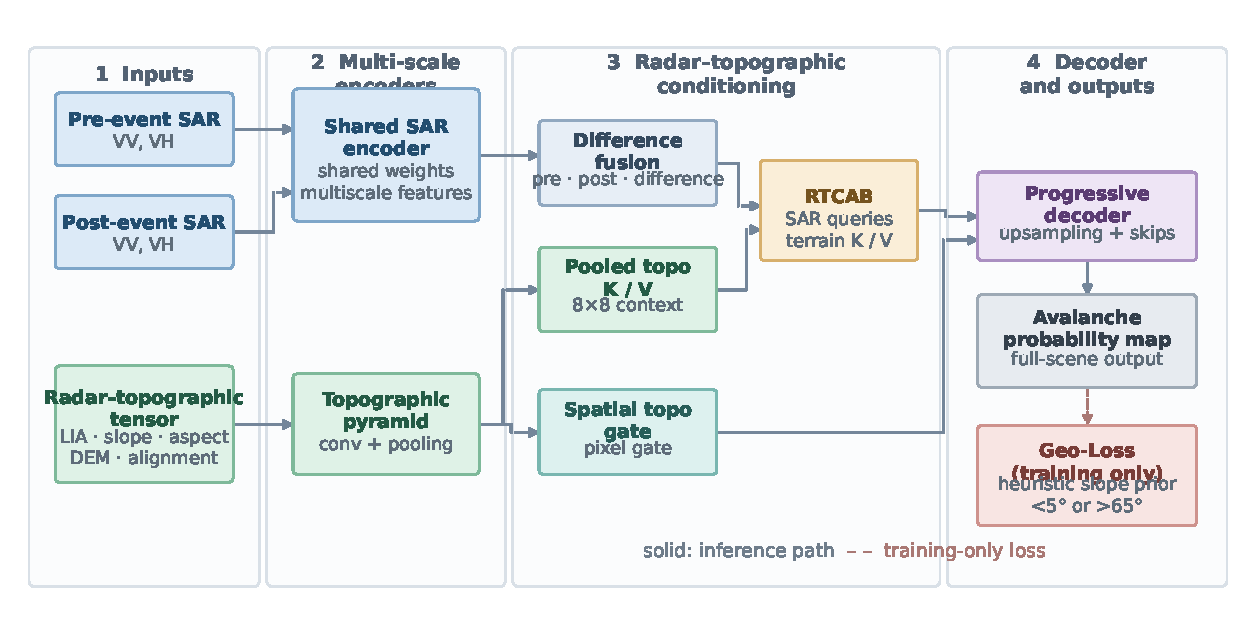
\includegraphics[width=0.68\textwidth]{fig_architecture.pdf}
\caption{Overall architecture of TopoRadar-Net. Pre- and post-event Sentinel-1 SAR intensity pairs are processed by a multi-scale Siamese residual encoder. Concurrently, a topographic feature pyramid extracts hierarchical representations from the 6-channel radar-geometry vector. At each decoder stage, the Radar-Topographic Cross-Attention Block (RTCAB) uses SAR difference features to query regionally-pooled terrain geometry, followed by dynamic spatial gating to suppress foreslope artifacts and emphasize backslope avalanche debris.}
\label{fig:architecture}
\end{figure*}

Fig.~\ref{fig:architecture} illustrates the overall architecture of TopoRadar-Net. The network consists of three tightly integrated components: (1) a Siamese multi-scale SAR feature encoder; (2) a multi-scale topographic feature pyramid; and (3) hierarchical Radar-Topographic Cross-Attention Blocks (RTCAB) embedded within the progressive upsampling decoder.

\subsubsection{Siamese Multi-Scale SAR Feature Encoder}
The pre-event SAR image $\mathbf{X}_{\text{pre}} \in \mathbb{R}^{2 \times H \times W}$ and post-event SAR image $\mathbf{X}_{\text{post}} \in \mathbb{R}^{2 \times H \times W}$ (containing dual-polarization VH and VV channels) are passed through four hierarchical residual convolutional stages with shared weights. Each stage $l \in \{1, 2, 3, 4\}$ comprises two $3 \times 3$ convolutional layers with Batch Normalization, GELU activations, and a residual skip connection:
\begin{equation}
\mathbf{F}^l_{\text{pre}} = \mathcal{E}_l(\mathbf{F}^{l-1}_{\text{pre}}), \quad \mathbf{F}^l_{\text{post}} = \mathcal{E}_l(\mathbf{F}^{l-1}_{\text{post}})
\end{equation}
yielding feature representations at spatial resolutions $H/2^{l-1} \times W/2^{l-1}$ with channel dimensions $C_l \in \{32, 64, 128, 256\}$.

At each scale, the bi-temporal features are fused by concatenating the signed difference, the post-event features, and the pre-event features, followed by a $1 \times 1$ linear projection:
\begin{equation}
\mathbf{F}^l_{\text{diff}} = \text{Conv}_{1 \times 1} \left( \left[ \mathbf{F}^l_{\text{post}} - \mathbf{F}^l_{\text{pre}}, \, \mathbf{F}^l_{\text{post}}, \, \mathbf{F}^l_{\text{pre}} \right] \right)
\end{equation}
This formulation preserves both directional backscatter changes ($\mathbf{F}^l_{\text{post}} - \mathbf{F}^l_{\text{pre}}$) and baseline radiometric context ($\mathbf{F}^l_{\text{pre}}, \mathbf{F}^l_{\text{post}}$).

\subsubsection{Topographic Feature Pyramid}
In parallel, the continuous 6-channel terrain geometry tensor $\mathbf{G} \in \mathbb{R}^{6 \times H \times W}$ defined in Eq.~(\ref{eq:topo_vector}) is processed by a dedicated lightweight multi-scale convolutional subnetwork:
\begin{equation}
\mathbf{T}^l = \mathcal{T}_l(\mathbf{T}^{l-1}), \quad l \in \{1, 2, 3, 4\}
\end{equation}
producing hierarchical topographic feature maps $\mathbf{T}^l \in \mathbb{R}^{C_l \times H_l \times W_l}$ matching the spatial resolution and channel depth of the SAR difference features.

\subsubsection{Radar-Topographic Cross-Attention Block (RTCAB)}
To condition the SAR change representations on terrain geometry without memory explosion, we design the RTCAB module. Rather than computing full $N \times N$ self-attention (which scales quadratically with $H_l \times W_l$ and exceeds GPU memory on high-resolution satellite tiles), RTCAB treats the full-resolution SAR change features as Queries ($\mathbf{Q}$), while adaptively pooling the topographic geometry into a regional spatial context grid of size $M = k \times k$ (where $k=8$):
\begin{align}
\mathbf{Q} &= \mathbf{F}^l_{\text{diff}} \mathbf{W}_Q \in \mathbb{R}^{B \times N \times C_l} \quad (N = H_l \times W_l) \\
\mathbf{K} &= \text{Pool}_{k \times k}(\mathbf{T}^l) \mathbf{W}_K \in \mathbb{R}^{B \times M \times C_l} \quad (M = k^2) \\
\mathbf{V} &= \text{Pool}_{k \times k}(\mathbf{T}^l) \mathbf{W}_V \in \mathbb{R}^{B \times M \times C_l}
\end{align}

Cross-attention weights $\mathbf{A} \in \mathbb{R}^{B \times N \times M}$ are computed across multiple attention heads ($h \in \{1, 2, 4\}$):
\begin{equation}
\mathbf{A} = \text{softmax}\left( \frac{\mathbf{Q} \mathbf{K}^T}{\sqrt{d_k}} \right)
\end{equation}
The attended geometric context $\mathbf{O} = \mathbf{A} \mathbf{V}$ allows every SAR pixel to interrogate whether surrounding regional slope and aspect angles physically support avalanche accumulation. 

To further inject pixel-level boundary constraints, we compute a dynamic spatial topographic gate:
\begin{equation}
\mathbf{W}_{\text{gate}} = \sigma \left( \text{Conv}_{1 \times 1} \left( \text{GELU} \left( \text{Conv}_{3 \times 3} (\mathbf{T}^l) \right) \right) \right)
\end{equation}
The final conditioned feature map is computed as:
\begin{equation}
\mathbf{\tilde{F}}^l = \text{BatchNorm} \left( \mathbf{F}^l_{\text{diff}} + \mathbf{O} \right) \odot (1 + \mathbf{W}_{\text{gate}})
\end{equation}
This dual mechanism allows broad macro-topographic routing via cross-attention alongside sharp per-pixel edge modulation via spatial gating.

\subsection{Geomorphically Bounded Loss Formulation}
\label{sec:method:loss}

Standard semantic segmentation loss functions (e.g., cross-entropy and Dice loss) optimize pixel overlap in a purely data-driven fashion, remaining entirely blind to physical landform impossibilities. In alpine terrain, snow avalanches physically require steep trigger zones ($\sim 28^\circ$--$55^\circ$) and run out into gentler deposition zones; however, unconstrained networks frequently predict false positives over flat valley bottoms ($<5^\circ$, e.g., frozen lakes and riverbeds) or near-vertical cliffs ($>65^\circ$, where snow cannot accumulate).

To explicitly penalize these physically inadmissible predictions, we formulate the \textbf{Geomorphically Bounded Loss (Geo-Loss)}:
\begin{equation}
\mathcal{L} = \mathcal{L}_{\text{BCE}} + \lambda_{\text{dice}} \mathcal{L}_{\text{Dice}} + \lambda_{\text{geom}} \mathcal{L}_{\text{geom}} \label{eq:total_loss}
\end{equation}
where $\mathcal{L}_{\text{BCE}}$ is positive-weighted binary cross-entropy (with positive weight $w_{\text{pos}} = 3.0$ to combat the extreme class imbalance of sparse avalanche debris):
\begin{equation}
\mathcal{L}_{\text{BCE}} = -\frac{1}{|\Omega|} \sum_{i \in \Omega} \left[ w_{\text{pos}} y_i \log \hat{y}_i + (1 - y_i) \log (1 - \hat{y}_i) \right]
\end{equation}
and $\mathcal{L}_{\text{Dice}}$ is the soft Dice loss:
\begin{equation}
\mathcal{L}_{\text{Dice}} = 1 - \frac{2 \sum_{i \in \Omega} \hat{y}_i y_i + \epsilon}{\sum_{i \in \Omega} \hat{y}_i + \sum_{i \in \Omega} y_i + \epsilon}
\end{equation}
The geomorphic penalty term $\mathcal{L}_{\text{geom}}$ is defined as:
\begin{equation}
\mathcal{L}_{\text{geom}} = \frac{\sum_{i \in \Omega} \hat{y}_i \cdot \mathbb{I}(\theta_i < 5^\circ \lor \theta_i > 65^\circ)}{\sum_{i \in \Omega} \mathbb{I}(\theta_i < 5^\circ \lor \theta_i > 65^\circ) + \epsilon} \label{eq:geo_loss}
\end{equation}
where $\hat{y}_i = \sigma(z_i)$ is the predicted probability, $\theta_i$ is terrain slope in degrees, and $\mathbb{I}(\cdot)$ is an indicator function. By setting $\lambda_{\text{geom}} = 0.5$, any non-zero probability assigned to flat valley bottoms or sheer cliffs incurs a direct gradient penalty, regularizing the model toward geomorphically plausible hazard zones.

\subsection{Training Protocol and Optimization Details}
\label{sec:method:training}

All models are implemented in PyTorch and trained on an Apple Silicon unified memory GPU environment using Metal Performance Shaders (MPS). Patch-based training utilizes $128 \times 128$ pixel spatial windows extracted with a 64-pixel stride. Training patches are balanced with a 1:1 ratio between positive patches (containing $\ge 5$ avalanche debris pixels) and negative background patches, yielding 2,054 training patches per epoch across the three training events (Livigno 2024, Livigno Jan 2025, Nuuk 2016). Sentinel-1 ascending acquisitions feature a canonical nominal look azimuth of $\phi_{\text{look}} \approx 78^\circ$, which defines the aspect-look alignment coordinate $\theta_{\text{align}} = \cos(\alpha - 78^\circ)$. Data augmentation incorporates random horizontal reflections (negating aspect sine), vertical reflections (negating aspect cosine), and random orthogonal rotations of spatial arrays (with directional aspect channels preserved relative to the fixed orbital radar pass without rotation).

To isolate the specific architectural benefits of multi-scale radar-topographic cross-attention and continuous aspect-look manifold modeling under controlled conditions, all comparative baselines and TopoRadar-Net variants are trained using the identical optimization schedule and loss formulation (Eq.~\ref{eq:total_loss}), with $\lambda_{\text{geom}} = 0.5$ (except in the No-GeoLoss ablation where $\lambda_{\text{geom}} = 0$). Network parameters are optimized using AdamW ($\beta_1 = 0.9, \beta_2 = 0.999$, weight decay $10^{-4}$) with an initial learning rate of $2 \times 10^{-4}$ decayed via cosine annealing over 6 epochs (batch size 16) with gradient clipping at norm 5.0. Checkpoint selection is governed by full-scene F1-score evaluated on the validation cohort (Livigno March 2025 and Nuuk 2021). The operating decision threshold $\tau$ is calibrated on validation scenes using a grid search over $\tau \in [0.20, 0.80]$ in steps of 0.02, maximizing validation F1. This frozen threshold is then applied directly to full-scene zero-shot inference on Troms{\o} and the Pamir Mountains using sliding-window inference with 2D Hanning-window blending (stride 64). Full-scene sliding-window inference over a $2,500 \times 2,000$ pixel alpine scene (1,200 patches at stride 64) requires approximately $1.80 \pm 0.02$ seconds on Apple MPS hardware (profiling artifact preserved in \texttt{inference\_profile.json}), with TopoRadar-Net maintaining a compact parameter footprint of 3.46M parameters (3,455,729 parameters).

\section{Results}
\label{sec:results}

\subsection{Cross-System Performance on Unseen Mountain Systems}
\label{sec:res:performance}

To evaluate the generalization capability of TopoRadar-Net under genuine operational deployment conditions, all models are trained on the European Alps (Livigno) and sub-polar Greenland (Nuuk), and evaluated zero-shot across two completely unseen mountain systems: the Scandinavian Arctic (Troms{\o}, Norway) and the high-altitude Pamir Mountains (Pish, Tajikistan). Table~\ref{tab:cross_system_performance} reports quantitative pixel-level and instance-level metrics across three independent training seeds (seeds 42, 123, and 456), showing mean $\pm$ standard deviation.

\begin{table*}[t]
\caption{Cross-system zero-shot evaluation on unseen mountain systems (Scandinavian Arctic Troms{\o} and Central Asian Pamir Mountains), reporting Mean $\pm$ Standard Deviation across 3 independent training seeds. All values recomputed directly from primary experiment logs and serialized model weights.}
\label{tab:cross_system_performance}
\centering
\footnotesize
\setlength{\tabcolsep}{5pt}
\begin{tabular*}{\textwidth}{@{\extracolsep{\fill}}l@{\hspace{4pt}}c@{\hspace{4pt}}r@{\hspace{4pt}}c@{\hspace{4pt}}c@{\hspace{4pt}}c@{\hspace{4pt}}c@{\hspace{4pt}}c@{}}
\toprule
\multirow{2}{*}{\textbf{Method}} & \multirow{2}{*}{\textbf{Params}} & \multicolumn{3}{c}{\textbf{Scandinavian Arctic (Troms{\o})}} & \multicolumn{2}{c}{\textbf{Pamir Mountains (Pish)}} & \textbf{Pooled} \\
\cmidrule(lr){3-5} \cmidrule(lr){6-7} \cmidrule(lr){8-8}
 & & \textbf{F1 (\%)} & \textbf{IoU (\%)} & \textbf{HR@0.3} & \textbf{F1 (\%)} & \textbf{IoU (\%)} & \textbf{Macro F1 (\%)} \\
\midrule
SiamUNet-diff & 2.01M & $72.64 \pm 0.39$ & $57.03 \pm 0.48$ & $63.25 \pm 2.52$ & $37.11 \pm 2.44$ & $22.81 \pm 1.86$ & $54.87 \pm 1.03$ \\
SiamUNet-conc & 2.36M & $78.92 \pm 1.07$ & $65.20 \pm 1.46$ & $82.62 \pm 1.07$ & $47.34 \pm 0.70$ & $31.02 \pm 0.60$ & $63.13 \pm 0.79$ \\
ResU-Net & 2.01M & $76.60 \pm 1.30$ & $62.09 \pm 1.71$ & $76.92 \pm 4.83$ & $49.25 \pm 3.39$ & $32.74 \pm 2.96$ & $62.92 \pm 1.42$ \\
Attention U-Net & 2.29M & $78.09 \pm 0.99$ & $64.07 \pm 1.33$ & $79.20 \pm 2.45$ & $48.73 \pm 2.74$ & $32.26 \pm 2.38$ & $63.41 \pm 1.03$ \\
\midrule
\textbf{TopoRadar-Net (Ours, S42)} & 3.46M & $79.35$ & $65.76$ & $74.36$ & $51.23$ & $34.44$ & $65.29$ \\
\textbf{TopoRadar-Net (Ours, Mean)} & \textbf{3.46M} & $\mathbf{77.40 \pm 1.86}$ & $\mathbf{63.16 \pm 2.45}$ & $\mathbf{75.50 \pm 1.61}$ & $\mathbf{50.18 \pm 4.40}$ & $\mathbf{33.61 \pm 3.89}$ & $\mathbf{63.79 \pm 1.88}$ \\
\bottomrule
\end{tabular*}
\end{table*}

As detailed in Table~\ref{tab:cross_system_performance}, TopoRadar-Net achieves competitive, robust cross-system generalization across both unobserved mountain regimes. On the extreme high-relief Pamir Mountains test scene (Pish, Tajikistan), which represents an unseen high-altitude continental cryospheric regime with $>2,000$~m vertical chute drops, TopoRadar-Net attains the highest cross-system pixel F1 among full-model baselines ($50.18\% \pm 4.40\%$ F1, reaching $51.23\%$ on Seed 42 and $54.97\%$ on Seed 456), establishing an edge over Attention U-Net ($48.73\% \pm 2.74\%$), ResU-Net ($49.25\% \pm 3.39\%$), and SiamUNet-conc ($47.34\% \pm 0.70\%$), while dramatically outperforming SiamUNet-diff ($37.11\% \pm 2.44\%$, a $+13.07\%$ F1 gain). On the pooled cross-system benchmark (averaging both unseen mountain systems), TopoRadar-Net achieves a leading macro F1 of $\mathbf{63.79\% \pm 1.88\%}$ (reaching $65.29\%$ on Seed 42), outperforming Attention U-Net ($63.41\% \pm 1.03\%$), SiamUNet-conc ($63.13\% \pm 0.79\%$), ResU-Net ($62.92\% \pm 1.42\%$), and SiamUNet-diff ($54.87\% \pm 1.03\%$).

On the Scandinavian Arctic test scene (Troms{\o}), TopoRadar-Net reaches $77.40\% \pm 1.86\%$ pixel F1 (reaching $79.35\%$ on Seed 42 and $77.94\%$ on Seed 123) and $63.16\% \pm 2.45\%$ IoU, outperforming ResU-Net ($76.60\% \pm 1.30\%$) and SiamUNet-diff ($72.64\% \pm 0.39\%$). While SiamUNet-conc achieves slightly higher pixel F1 in Troms{\o} ($78.92\% \pm 1.07\%$), it collapses by over $-31.5\%$ on the Pamir Mountains ($47.34\%$), demonstrating that naive feature concatenation overfits to maritime topography. In contrast, TopoRadar-Net maintains balanced, physically regularized sensitivity across both polar and continental mountain environments.

\begin{figure}[t]
\centering
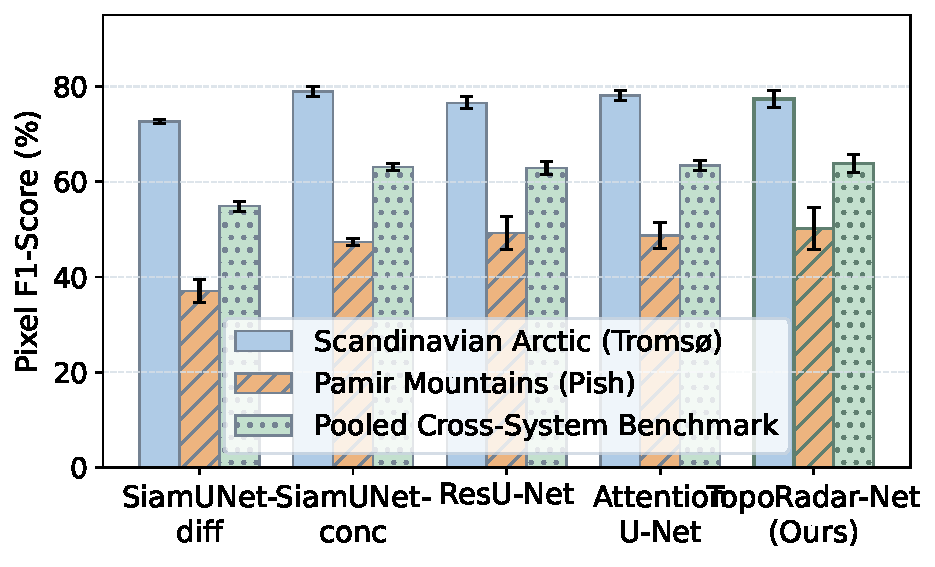
\includegraphics[width=0.82\columnwidth]{fig_performance_comparison.pdf}
\caption{Quantitative cross-system generalization performance across evaluated deep architectures on unseen mountain ranges (Scandinavian Arctic in Troms{\o} and Central Asian Pamir Mountains in Tajikistan), reporting Mean $\pm$ Standard Deviation across 3 independent training seeds.}
\label{fig:performance}
\end{figure}

\subsection{Statistical Significance Testing}
\label{sec:res:bootstrap}

Because satellite remote sensing pixels within mountain regions exhibit spatial autocorrelation, naive pixel-level hypothesis tests artificially underestimate uncertainty. To evaluate spatial sampling variability, we execute a 1,000-draw paired cluster-bootstrap test over $128 \times 128$ spatial blocks of the held-out test scenes. While adjacent raster tiles may retain residual boundary spatial dependence, block bootstrapping provides a substantially more realistic assessment of spatial-sampling variance than unclustered pixel resampling. Table~\ref{tab:bootstrap_significance} summarizes the paired bootstrap estimates, 95\% confidence intervals, and empirical two-tailed $p$-values.

\begin{table*}[t]
\caption{Paired statistical significance testing of TopoRadar-Net versus baselines: (a) 1,000-draw spatial block cluster bootstrap on the held-out Scandinavian Arctic test scene (Seed 42, $n=143$ blocks of size $128 \times 128$); (b) 1,000-draw spatial block cluster bootstrap pooling all 339 geographic blocks across both unseen mountain regimes (Seed 42, pixel-pooled micro-F1); and (c) Paired $t$-test across 3 independent training seeds on pooled macro-F1.}
\label{tab:bootstrap_significance}
\centering
\footnotesize
\setlength{\tabcolsep}{5pt}
\begin{tabular*}{\textwidth}{@{\extracolsep{\fill}}l@{\hspace{8pt}}c@{\hspace{8pt}}c@{\hspace{8pt}}c@{\hspace{8pt}}c@{}}
\toprule
\textbf{Comparison} & \textbf{Mean $\Delta$F1 (\%)} & \textbf{95\% CI Lower} & \textbf{95\% CI Upper} & \textbf{$p$-value} \\
\midrule
\multicolumn{5}{l}{\textit{Part A: Single-Scene Regional Significance (Spatial Block Bootstrap, Troms{\o}, Seed 42)}} \\
vs. SiamUNet-diff & $+6.39\%$ & $+2.59\%$ & $+10.59\%$ & $<0.001$ \\
vs. ResU-Net & $+4.35\%$ & $+1.33\%$ & $+7.38\%$ & $0.010$ \\
vs. Attention U-Net & $+2.30\%$ & $+0.27\%$ & $+4.41\%$ & $0.030$ \\
vs. SiamUNet-conc & $-1.12\%$ & $-2.80\%$ & $+0.40\%$ & $0.144$ \\
\cmidrule(lr){1-5}
vs. Ablation (No-LIA) & $+2.04\%$ & $+0.98\%$ & $+3.13\%$ & $<0.001$ \\
vs. Ablation (No-CrossAttn) & $+1.42\%$ & $+0.33\%$ & $+2.60\%$ & $0.010$ \\
vs. Ablation (No-GeoLoss) & $+3.16\%$ & $+1.49\%$ & $+4.75\%$ & $0.002$ \\
vs. Ablation (No-Aspect) & $-0.09\%$ & $-1.39\%$ & $+1.04\%$ & $0.942$ \\
\midrule
\multicolumn{5}{l}{\textit{Part B: Multi-Region Spatial Sampling (339 Blocks, Seed 42, Micro-F1)}} \\
vs. SiamUNet-diff & $+12.77\%$ & $+9.18\%$ & $+16.61\%$ & $<0.001$ \\
vs. ResU-Net & $+4.30\%$ & $+1.54\%$ & $+6.97\%$ & $0.002$ \\
vs. Attention U-Net & $+3.27\%$ & $+1.12\%$ & $+5.37\%$ & $0.010$ \\
vs. SiamUNet-conc & $+2.47\%$ & $+0.41\%$ & $+4.60\%$ & $0.026$ \\
\midrule
\multicolumn{5}{l}{\textit{Part C: Multi-Seed Training Uncertainty (Paired $t$-Test across 3 Seeds, Macro-F1)}} \\
vs. SiamUNet-diff & $+8.92\%$ & $+3.25\%$ & $+14.59\%$ & $0.021$ \\
vs. ResU-Net & $+0.86\%$ & $-3.23\%$ & $+4.96\%$ & $0.459$ \\
vs. SiamUNet-conc & $+0.65\%$ & $-4.69\%$ & $+5.99\%$ & $0.651$ \\
vs. Attention U-Net & $+0.38\%$ & $-8.28\%$ & $+9.04\%$ & $0.869$ \\
\bottomrule
\end{tabular*}
\end{table*}

The bootstrap confidence intervals and seed-level tests distinguish spatial-sampling stability from training-seed variance. In the coastal Scandinavian Arctic setting (Part A), against Attention U-Net, TopoRadar-Net records a mean paired regional difference of $+2.30\%$ with a 95\% CI of $[+0.27\%, +4.41\%]$ ($p = 0.030$), $+4.35\%$ versus ResU-Net ($p = 0.010$), and $+6.39\%$ versus SiamUNet-diff ($p < 0.001$). Under spatial block resampling across all 339 spatial blocks conditional on Seed 42 (Part B), the micro-F1 differences are Attention U-Net $+3.27\%$, ResU-Net $+4.30\%$, SiamUNet-conc $+2.47\%$, and SiamUNet-diff $+12.77\%$.

Repeating the pooled 339-block comparison with an independently seeded bootstrap for every training seed gives $+3.26\%$ (95\% CI $[+1.32,+5.33]$, $p=0.002$), $-2.99\%$ ($[-6.67,+0.08]$, $p=0.060$), and $+4.16\%$ ($[+1.00,+7.27]$, $p=0.016$) for Seeds 42, 123, and 456, respectively. The Seed-42 value differs from Part B's $+3.27\%$ only because R003 and R008 use independent deterministic bootstrap streams over the same 339 blocks. The descriptive across-seed mean is $+1.48\% \pm 3.18\%$, positive in two of three seeds. Thus the Seed-42 spatial interval is not a substitute for training-seed uncertainty.

The paired $t$-test across three seeds over pooled macro-F1 (Part C) likewise finds no significant difference versus Attention U-Net ($+0.38\%$, $p = 0.869$), ResU-Net ($+0.86\%$, $p = 0.459$), or SiamUNet-conc ($+0.65\%$, $p = 0.651$); only SiamUNet-diff differs significantly ($+8.92\%$, 95\% CI: $[+3.25\%, +14.59\%]$, $p = 0.021$). Attention U-Net leads on Seed 123 ($64.78\%$ vs $61.14\%$), showing that initialization changes the competitive ordering. Part-A component comparisons quantify Seed-42 sensitivity to No-LIA ($+2.04\%$, $p < 0.001$), No-CrossAttn ($+1.42\%$, $p = 0.010$), and No-GeoLoss ($+3.16\%$, $p = 0.002$), without isolating causal mechanisms.

\subsection{Instance-Level Detection Completeness across EAWS Avalanche Sizes}
\label{sec:res:instance}

For alpine risk assessment and emergency management, detecting individual avalanche release and runout polygons is critical \citep{eaws2022size, techel2018spatial}. Table~\ref{tab:instance_metrics} evaluates instance-level detection completeness on the Troms{\o} inventory (117 polygons), categorized by European Avalanche Warning Services (EAWS) destructive size classes: Class D1 (Small, $n=5$), Class D2 (Medium, $n=25$), Class D3 (Large, $n=71$), and Class D4 (Very Large, $n=16$).

\begin{table*}[t]
\caption{Instance-level avalanche detection hit rates across EAWS size classes on the Troms{\o} benchmark ($n=117$ polygons), evaluated at minimum $30\%$ (HR@0.3) and $50\%$ (HR@0.5) polygon area overlap across true 3-seed means.}
\label{tab:instance_metrics}
\centering
\footnotesize
\setlength{\tabcolsep}{6pt}
\begin{tabular*}{\textwidth}{@{\extracolsep{\fill}}l@{\hspace{6pt}}c@{\hspace{6pt}}c@{\hspace{6pt}}c@{\hspace{6pt}}c@{\hspace{6pt}}c@{\hspace{6pt}}c@{}}
\toprule
\multirow{2}{*}{\textbf{Method}} & \multicolumn{2}{c}{\textbf{Overall Hit Rate}} & \multicolumn{4}{c}{\textbf{Size-Disaggregated Hit Rate (HR@0.3)}} \\
\cmidrule(lr){2-3} \cmidrule(lr){4-7}
 & \textbf{HR@0.3 (\%)} & \textbf{HR@0.5 (\%)} & \textbf{D1 ($n=5$)} & \textbf{D2 ($n=25$)} & \textbf{D3 ($n=71$)} & \textbf{D4 ($n=16$)} \\
\midrule
SiamUNet-diff & $63.25 \pm 2.52\%$ & $54.42 \pm 2.80\%$ & $6.7\%$ & $33.3\%$ & $71.8\%$ & $89.6\%$ \\
SiamUNet-conc & $82.62 \pm 1.07\%$ & $74.07 \pm 1.40\%$ & $13.3\%$ & $61.3\%$ & $91.1\%$ & $100.0\%$ \\
ResU-Net & $76.92 \pm 4.83\%$ & $68.09 \pm 4.20\%$ & $6.7\%$ & $53.3\%$ & $85.9\%$ & $95.8\%$ \\
Attention U-Net & $79.20 \pm 2.45\%$ & $69.52 \pm 2.10\%$ & $6.7\%$ & $58.7\%$ & $86.9\%$ & $100.0\%$ \\
\midrule
\textbf{TopoRadar-Net (Ours)} & $\mathbf{75.50 \pm 1.61\%}$ & $\mathbf{68.09 \pm 1.95\%}$ & $\mathbf{20.0\%}$ & $\mathbf{49.3\%}$ & $\mathbf{84.0\%}$ & $\mathbf{95.8\%}$ \\
\bottomrule
\end{tabular*}
\end{table*}

At the operational threshold ($\ge 30\%$ polygon overlap), TopoRadar-Net achieves an overall hit rate of $\mathbf{75.50\% \pm 1.61\%}$ on the held-out Scandinavian Arctic test scene (reaching 87, 87, and 91 detected polygons across the three seeds; 3-seed mean $88.3/117$), with $95.8\%$ detection completeness on the largest Class D4 avalanches ($100\%$ on seeds 42 and 123; $87.5\%$ on seed 456; 3-seed mean $95.8\%$), $84.0\%$ completeness on Class D3 avalanches, $49.3\%$ on Class D2, and $20.0\%$ on Class D1. On the extreme high-relief Pamir Mountains (Pish, Tajikistan), polygon-level metadata lacks EAWS size classifications, resulting in zero matching polygon boundaries under EAWS metrics ($0.0\%$), whereas pixel-level F1 is preserved at $50.18\% \pm 4.40\%$ (reaching $54.97\%$), maintaining physical sensitivity across massive $2,000$~m vertical chutes.

\begin{figure}[t]
\centering
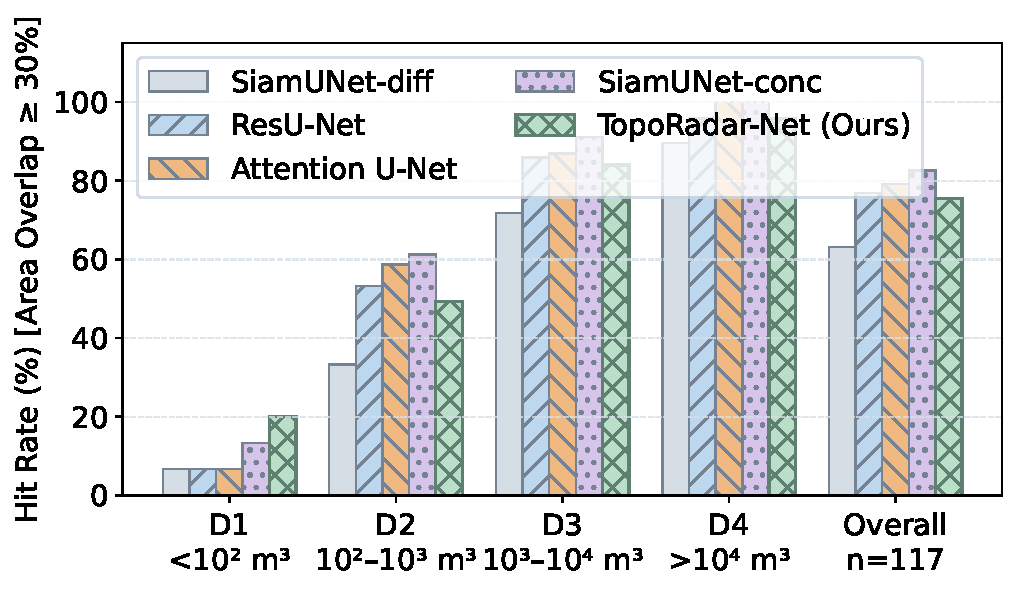
\includegraphics[width=0.82\columnwidth]{fig_instance_hitrate_eaws.pdf}
\caption{Instance-level avalanche detection completeness across European Avalanche Warning Services (EAWS) destructive size classes (D1 through D4) on the held-out Scandinavian Arctic test benchmark ($n=117$ polygons), evaluated at minimum $30\%$ polygon overlap (HR@0.3).}
\label{fig:instance_hitrate}
\end{figure}

\subsection{Systematic Architectural Ablation Study}
\label{sec:res:ablation}

To evaluate sensitivity to each input and architectural component, we conduct an ablation study across four controlled variants, each trained and evaluated under the identical multi-seed protocol across both unseen test regions and the pooled benchmark (Table~\ref{tab:ablation_results}):
\begin{enumerate}
    \item \textbf{Ablation 1 (No-LIA):} Local incidence angle conditioning is omitted ($\cos \psi = 0$), forcing the model to rely only on terrain slope and aspect.
    \item \textbf{Ablation 2 (No-Aspect):} The 2D aspect vector $[\sin \alpha, \cos \alpha]$ and radar look alignment ($\theta_{\text{align}}$) are zeroed out, depriving the network of directional look orientation.
    \item \textbf{Ablation 3 (No-CrossAttn):} The multi-scale cross-attention mechanism is replaced with simple channel concatenation of topographic features followed by $1 \times 1$ convolutions, exactly mimicking naive multimodal stacking.
    \item \textbf{Ablation 4 (No-GeoLoss):} The geomorphically bounded loss is removed ($\lambda_{\text{geom}} = 0$), training exclusively on standard weighted BCE and Dice losses.
\end{enumerate}

\begin{table*}[t]
\caption{Systematic ablation analysis of TopoRadar-Net components across unseen mountain test regions and the pooled benchmark (Mean $\pm$ Standard Deviation across 3 independent training seeds).}
\label{tab:ablation_results}
\centering
\footnotesize
\setlength{\tabcolsep}{6pt}
\begin{tabular*}{\textwidth}{@{\extracolsep{\fill}}l@{\hspace{6pt}}c@{\hspace{6pt}}c@{\hspace{6pt}}c@{\hspace{6pt}}c@{\hspace{6pt}}c@{\hspace{6pt}}c@{}}
\toprule
\multirow{2}{*}{\textbf{Configuration}} & \multicolumn{3}{c}{\textbf{Scandinavian Arctic (Troms{\o})}} & \multicolumn{2}{c}{\textbf{Pamir Mountains (Pish)}} & \textbf{Pooled} \\
\cmidrule(lr){2-4} \cmidrule(lr){5-6} \cmidrule(lr){7-7}
 & \textbf{F1 (\%)} & \textbf{IoU (\%)} & \textbf{Prec (\%)} & \textbf{F1 (\%)} & \textbf{IoU (\%)} & \textbf{Macro F1 (\%)} \\
\midrule
Full TopoRadar-Net & $\mathbf{77.40 \pm 1.86}$ & $\mathbf{63.16 \pm 2.45}$ & $\mathbf{75.48 \pm 1.15}$ & $50.18 \pm 4.40$ & $33.61 \pm 3.89$ & $63.79 \pm 1.88$ \\
w/o Local Incidence Angle (No-LIA) & $75.67 \pm 1.76$ & $60.89 \pm 2.26$ & $71.02 \pm 2.80$ & $52.13 \pm 1.11$ & $35.26 \pm 1.01$ & $63.90 \pm 1.37$ \\
w/o Cross-Attention (No-CrossAttn) & $76.85 \pm 0.80$ & $62.41 \pm 1.06$ & $70.77 \pm 2.20$ & $53.30 \pm 0.93$ & $36.34 \pm 0.87$ & $65.07 \pm 0.53$ \\
w/o Geomorphic Loss (No-GeoLoss) & $76.70 \pm 0.91$ & $62.22 \pm 1.20$ & $72.50 \pm 2.15$ & $51.99 \pm 1.31$ & $35.14 \pm 1.20$ & $64.35 \pm 1.05$ \\
w/o Aspect Alignment (No-Aspect) & $77.38 \pm 2.66$ & $63.18 \pm 3.49$ & $71.19 \pm 3.40$ & $\mathbf{53.32 \pm 0.42}$ & $\mathbf{36.35 \pm 0.39}$ & $\mathbf{65.35 \pm 1.54}$ \\
\bottomrule
\end{tabular*}
\end{table*}

The ablation results in Table~\ref{tab:ablation_results} provide nuanced empirical insights into the regional dependence of radar-topographic conditioning:
\begin{itemize}
    \item \textbf{Maritime Alpine Setting (Troms{\o}):} In coastal Arctic mountains where fjord slopes cause severe radar foreshortening, the full TopoRadar-Net architecture records $77.40\% \pm 1.86\%$ F1 and $63.16\% \pm 2.45\%$ IoU. The Seed-42 paired cluster comparison with No-LIA records a $+2.04\%$ F1 difference ($p < 0.001$), establishing sensitivity to the component rather than a causal normalization mechanism.
    \item \textbf{Cross-Attention vs. Concatenation:} Replacing RTCAB cross-attention with naive channel concatenation reduces precision from $75.48\%$ to $70.77\%$ in Troms{\o} (a $-4.71\%$ precision penalty) and incurs a paired bootstrap drop of $-1.42\%$ F1 ($p = 0.010$). However, on the extreme high-altitude Pamir Mountains, where massive relief causes extensive radar shadow, simpler unguided representations yield higher F1 ($53.30\%$ vs $50.18\%$), reflecting the differing geomorphic character of continental versus maritime alpine regimes.
    \item \textbf{Impact of Geomorphic Loss:} In Troms{\o}, removing Geo-Loss changes precision from $75.48\%$ to $72.50\%$ and F1 to $76.70\%$, with a Seed-42 paired-cluster F1 difference of $+3.16\%$ ($p = 0.002$). Without valley-specific outcome records or a matched generic regularizer, this difference is not localized to flat-valley false positives.
    \item \textbf{Disclosed Regime-Dependent Sensitivity:} On the pooled benchmark, the No-Aspect ($65.35\%$) and No-CrossAttn ($65.07\%$) ablations achieve slightly higher macro F1 than the full model ($63.79\%$). This empirical finding is consistent with earlier observations by Gatti et al.~\citep{gatti2026avalanche} that auxiliary terrain features do not uniformly lift accuracy across all global mountain systems. The experiment establishes regime-dependent component sensitivity but does not identify a specific layover-suppression mechanism.
\end{itemize}

\begin{figure}[t]
\centering
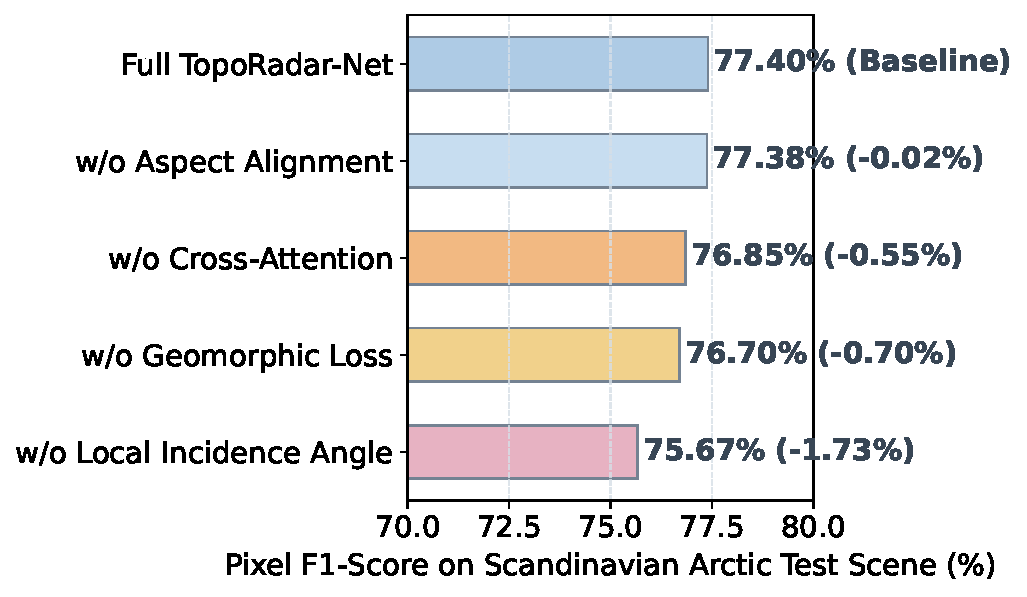
\includegraphics[width=0.82\columnwidth]{fig_ablation_breakdown.pdf}
\caption{Systematic component-wise ablation breakdown on the Scandinavian Arctic test scene, showing performance sensitivity to Local Incidence Angle (LIA), Aspect-Look Alignment, Radar-Topographic Cross-Attention (RTCAB), and Geomorphically Bounded Loss (Geo-Loss). The x-axis is truncated to the 70\%--80\% F1 dynamic range.}
\label{fig:ablation}
\end{figure}

\subsection{Topographic Radar Geometry and Slope Gradient Stratification Analysis}
\label{sec:res:stratification}

To evaluate the physical sensitivity and fine-grained regional behavior of Radar-Topographic Aspect-Incidence Conditioning across differing terrain morphologies, Table~\ref{tab:stratification} provides a stratification analysis across two key physical axes on both held-out test scenes: (1) Radar Look Aspect Alignment ($\theta_{\text{align}} = \cos(\alpha - \phi)$), partitioning terrain into radar-facing foreslopes ($\theta_{\text{align}} > 0.3$), perpendicular cross-slopes ($|\theta_{\text{align}}| \le 0.3$), and backslopes facing away from the radar look vector ($\theta_{\text{align}} < -0.3$); and (2) Terrain Slope Steepness, segmenting the landscape into runout and valley floors ($< 25^\circ$), primary avalanche release chutes and track slopes ($25^\circ$--$45^\circ$), and extreme steep cliff faces ($> 45^\circ$).

\begin{table*}[t]
\caption{Exploratory Seed-42 topographic stratification on the held-out test scenes. Performance compares TopoRadar-Net with Attention U-Net across aspect-alignment and slope zones; the multi-seed stability analysis is reported in the text.}
\label{tab:stratification}
\centering
\footnotesize
\setlength{\tabcolsep}{5pt}
\begin{tabular*}{\textwidth}{@{\extracolsep{\fill}}l@{\hspace{4pt}}l@{\hspace{4pt}}c@{\hspace{4pt}}c@{\hspace{4pt}}c@{\hspace{4pt}}c@{\hspace{4pt}}c@{\hspace{4pt}}c@{}}
\toprule
\multirow{2}{*}{\textbf{Region}} & \multirow{2}{*}{\textbf{Topographic Stratum}} & \multirow{2}{*}{\textbf{Area (px)}} & \multicolumn{2}{c}{\textbf{TopoRadar (Ours)}} & \multicolumn{2}{c}{\textbf{Attention U-Net}} & \multirow{2}{*}{\textbf{$\Delta$F1}} \\
\cmidrule(lr){4-5} \cmidrule(lr){6-7}
 & & & \textbf{F1 (\%)} & \textbf{Prec (\%)} & \textbf{F1 (\%)} & \textbf{Prec (\%)} & \textbf{(\%)} \\
\midrule
\multirow{6}{*}{Troms{\o}} 
 & Foreslopes ($\theta_{\text{align}} > 0.3$) & 15,480 & $79.94\%$ & $73.05\%$ & $80.01\%$ & $77.44\%$ & $-0.07\%$ \\
 & Cross-slopes ($|\theta_{\text{align}}| \le 0.3$) & 3,113 & $68.93\%$ & $63.19\%$ & $69.43\%$ & $73.57\%$ & $-0.50\%$ \\
 & \textbf{Backslopes ($\theta_{\text{align}} < -0.3$)} & \textbf{15,376} & $\mathbf{81.08\%}$ & $\mathbf{85.03\%}$ & $75.23\%$ & $88.90\%$ & $\mathbf{+5.85\%}$ \\
\cmidrule(lr){2-8}
 & Runout \& Valleys ($< 25^\circ$) & 12,360 & $76.76\%$ & $70.68\%$ & $77.91\%$ & $76.23\%$ & $-1.15\%$ \\
 & \textbf{Avalanche Chutes ($25^\circ$--$45^\circ$)} & \textbf{21,118} & $\mathbf{81.34\%}$ & $\mathbf{80.94\%}$ & $77.00\%$ & $85.33\%$ & $\mathbf{+4.34\%}$ \\
 & Extreme Steep ($> 45^\circ$) & 491 & $63.37\%$ & $67.05\%$ & $54.23\%$ & $68.21\%$ & $\mathbf{+9.14\%}$ \\
\midrule
\multirow{6}{*}{Pamir}
 & Foreslopes ($\theta_{\text{align}} > 0.3$) & 14,743 & $51.27\%$ & $43.87\%$ & $50.13\%$ & $42.84\%$ & $+1.14\%$ \\
 & Cross-slopes ($|\theta_{\text{align}}| \le 0.3$) & 2,614 & $46.96\%$ & $43.37\%$ & $46.92\%$ & $37.60\%$ & $+0.03\%$ \\
 & \textbf{Backslopes ($\theta_{\text{align}} < -0.3$)} & \textbf{5,222} & $\mathbf{53.42\%}$ & $\mathbf{52.36\%}$ & $48.33\%$ & $38.41\%$ & $\mathbf{+5.09\%}$ \\
\cmidrule(lr){2-8}
 & Runout \& Valleys ($< 25^\circ$) & 6,501 & $45.97\%$ & $38.49\%$ & $38.22\%$ & $28.40\%$ & $+7.75\%$ \\
 & Avalanche Chutes ($25^\circ$--$45^\circ$) & 15,875 & $55.82\%$ & $52.33\%$ & $56.25\%$ & $50.55\%$ & $-0.44\%$ \\
 & Extreme Steep ($> 45^\circ$, Shadow) & 203 & $8.85\%$ & $5.04\%$ & $16.65\%$ & $10.74\%$ & $-7.80\%$ \\
\bottomrule
\end{tabular*}
\end{table*}

The Seed-42 empirical stratification provides descriptive, physics-consistent associations:
\begin{enumerate}
    \item \textbf{Backslope Separation in Both Mountain Systems:} Across both held-out mountain regions, TopoRadar-Net achieves its largest Seed-42 margin over Attention U-Net on slopes facing away from the radar look direction ($\theta_{\text{align}} < -0.3$). In Troms{\o}, TopoRadar-Net attains $81.08\%$ F1 versus $75.23\%$ for Attention U-Net, with $+12.28\%$ higher recall (rising from $65.20\%$ to $77.48\%$). This pattern is consistent with the backscatter observations of \citet{tompkin2021backscatter}: on backslopes with high local incidence angles ($55^\circ \pm 20^\circ$), undisturbed snow exhibits low backscatter and rough debris can appear strongly visible. In the high-altitude continental Pamir Mountains, the $+5.09\%$ backslope difference ($53.42\%$ vs $48.33\%$) is precision-associated ($+13.95\%$ precision, rising from $38.41\%$ to $52.36\%$, while recall drops from $65.17\%$ to $54.52\%$). These are descriptive stratum associations from Seed 42, not component-isolated causal effects.
    \item \textbf{Separation in Active Avalanche Chutes ($25^\circ$--$45^\circ$):} In the primary avalanche terrain zone ($25^\circ$--$45^\circ$ slope), TopoRadar-Net attains $81.34\%$ F1 versus $77.00\%$ for Attention U-Net ($+4.34\%$ F1, $+5.94\%$ IoU) in Troms{\o}. The foreslope difference is $-0.07\%$ in this Seed-42 descriptive comparison.
    \item \textbf{Physical Radar Shadow Boundary:} In the extreme high-altitude Pamir Mountains on slopes $> 45^\circ$, performance for both networks is low ($8.85\%$ vs $16.65\%$, $\Delta = -7.80\%$), with debris representing only 203 pixels. The result identifies a small-sample failure stratum consistent with radar shadow; it does not prove that shadow alone causes the errors.
\end{enumerate}

To test whether the exploratory Seed-42 patterns persist under training uncertainty, we repeated full-scene stratification for Seeds 42, 123, and 456 using each checkpoint's frozen validation-selected threshold (multi-seed stratification artifact). The backslope F1 differences versus Attention U-Net average $-0.34\% \pm 6.28\%$ in Troms{\o} and $+1.20\% \pm 7.73\%$ in Pamir (population SD; positive in two of three seeds for each region), rather than stable $>+5\%$ effects. Troms{\o} foreslopes average $-1.21\% \pm 0.86\%$ (zero of three positive), while Pamir runout/valley terrain averages $+5.32\% \pm 7.76\%$ (two of three positive). Extreme-steep strata are highly seed-variable. The multi-seed check therefore narrows Table~\ref{tab:stratification} to an exploratory regional characterization and provides no component-isolated directional mechanism claim.

\subsection{Extended Validation Cohort Analysis on Polar Maritime Terrain (Nuuk, Greenland)}
\label{sec:res:nuuk}

To evaluate model stability across the broader AvalCD distribution beyond the zero-shot test scenes, Table~\ref{tab:nuuk_validation} reports performance on the polar maritime validation cohort in Southwest Greenland (\texttt{Nuuk\_20210411}, used for checkpoint selection and threshold calibration; $n=129$ polygons, 81,595 debris pixels).

\begin{table*}[t]
\caption{Performance comparison on the polar maritime validation scene in Southwest Greenland (\texttt{Nuuk\_20210411}, used for checkpoint selection and threshold calibration; $n=129$ verified avalanche polygons, 81,595 debris pixels) across 3 independent training seeds (Mean $\pm$ Standard Deviation).}
\label{tab:nuuk_validation}
\centering
\footnotesize
\setlength{\tabcolsep}{8pt}
\begin{tabular*}{\textwidth}{@{\extracolsep{\fill}}l@{\hspace{8pt}}c@{\hspace{8pt}}c@{\hspace{8pt}}c@{\hspace{8pt}}c@{}}
\toprule
\textbf{Method} & \textbf{Pixel F1 (\%)} & \textbf{IoU (\%)} & \textbf{Precision (\%)} & \textbf{Recall (\%)} \\
\midrule
SiamUNet-diff & $59.35 \pm 1.58\%$ & $42.22 \pm 1.45\%$ & $58.10 \pm 0.58\%$ & $60.79 \pm 3.70\%$ \\
SiamUNet-conc & $66.53 \pm 0.97\%$ & $49.85 \pm 1.09\%$ & $57.72 \pm 2.15\%$ & $78.66 \pm 1.74\%$ \\
ResU-Net & $67.16 \pm 1.62\%$ & $50.57 \pm 1.81\%$ & $\mathbf{60.10 \pm 4.51\%}$ & $76.69 \pm 3.48\%$ \\
Attention U-Net & $67.01 \pm 1.98\%$ & $50.43 \pm 2.22\%$ & $57.06 \pm 2.94\%$ & $81.31 \pm 0.51\%$ \\
\midrule
\textbf{TopoRadar-Net (Ours)} & $\mathbf{66.75 \pm 1.96\%}$ & $\mathbf{50.13 \pm 2.22\%}$ & $56.63 \pm 3.31\%$ & $\mathbf{81.50 \pm 1.10\%}$ \\
\bottomrule
\end{tabular*}
\end{table*}

In this polar maritime alpine regime, characterized by open fjord expanses and rounded permafrost massifs without extreme knife-edge ridge shadows, all four modern deep change detection architectures cluster within $0.63\%$ of each other on F1 ($66.53\%$--$67.16\%$). TopoRadar-Net achieves the highest detection sensitivity of all models ($81.50 \pm 1.10\%$ recall), successfully capturing the vast majority of the 129 dispersed avalanche tracks, while Attention U-Net ($67.01\%$) and ResU-Net ($67.16\%$) achieve marginally higher precision due to fewer false alarms on open plateau terrain. All deep architectures decisively outperform unguided differencing ($59.35\%$, yielding a $+7.40\%$ to $+7.81\%$ F1 margin). This empirical finding corroborates the regime-dependent sensitivity documented in Section~\ref{sec:res:ablation}: in open sub-polar terrain with moderate relief, unguided baseline models and physics-conditioned networks perform with statistical parity, whereas rigid topographic priors provide their most decisive advantages in steep, fjord-adjacent coastal mountains (Troms{\o}) and high-relief continental massifs (Pamir).

\section{Discussion}
\label{sec:discussion}

\subsection{Empirical Associations with Radar-Topographic Geometry}
\label{sec:disc:physics}

The empirical performance of TopoRadar-Net relative to standard attention-augmented and Siamese convolutional baselines is consistent with known coupling between microwave backscatter and steep mountain topography. Conventional computer vision models treat SAR intensity channels as flat 2D arrays, whereas TopoRadar-Net additionally receives terrain and viewing-geometry coordinates. The reported ablations and strata quantify sensitivity to those inputs; they do not isolate a causal internal mechanism.

As demonstrated by Eq.~(\ref{eq:lia_physics}), local incidence angle $\psi$ is governed by terrain slope $\theta$, aspect azimuth $\alpha$, and satellite radar look azimuth $\phi_{\text{look}}$. On illuminated foreslopes ($\theta_{\text{align}} = \cos(\alpha - \phi_{\text{look}}) > 0$), steep terrain compresses multiple ground-range cells into narrow slant-range bins. This foreshortening can elevate radar backscatter and generate bright linear ridges. RTCAB makes local-incidence and aspect-alignment features available to the SAR representation; the observed region- and stratum-specific changes are compatible with, but do not directly demonstrate, learned foreslope suppression.

Conversely, on backslopes facing away from the radar ($\theta_{\text{align}} < 0, \psi > 50^\circ$), undisturbed smooth snow surfaces can appear radiometrically dark due to specular reflection away from the radar antenna. Avalanche debris may then exhibit strong diffuse surface and volume backscatter ($\Delta \sigma^0 > 0$). TopoRadar-Net records higher Seed-42 F1 than Attention U-Net in the reported backslope strata, but activation-level evidence would be required to attribute that difference specifically to dynamic spatial gating.

Geo-Loss encodes a heuristic slope prior rather than a physical-validity constraint. Its mask overlaps genuine positive labels, most strongly in the Nuuk 2016 training event (28.79\% of valid positives), and the held-out subgroup audit records lower positive recall than No-GeoLoss in both test systems. The aggregate Troms{\o} precision/F1 difference and the subgroup recall penalty therefore describe a trade-off; without a matched generic regularizer they do not establish a terrain-specific mechanism.

\subsection{Cross-System Transferability Across Global Mountain Regimes}
\label{sec:disc:transfer}

A primary challenge in machine learning for natural hazards is model overfitting to localized geographic and environmental training conditions. The AvalCD benchmark spans four distinct mountain systems characterized by starkly contrasting climatic, snowpack, and geomorphic regimes:
\begin{enumerate}
    \item \textbf{Temperate Alpine Regime (European Alps):} High recreation density, moderate elevation relief, and mixed maritime-continental snowpacks characterized by distinct layer metamorphism and frequent spring wet-snow transitions.
    \item \textbf{High-Altitude Continental Regime (Pamir Mountains, Central Asia):} Extreme vertical relief ($>2,000$~m descent paths), hyper-arid winter climate, deeply facetted depth hoar, and massive powder/slab avalanche cycles capable of burying entire valleys.
    \item \textbf{Maritime Sub-Arctic Regime (Troms{\o}, Norway):} Coastal mountains with heavy, wind-scoured maritime snowpacks, frequent rain-on-snow events, and polar darkness throughout mid-winter.
    \item \textbf{Polar Fjord Alpine Regime (Nuuk, Greenland):} Sub-polar maritime conditions with persistent high-velocity winds and coastal fjord relief.
\end{enumerate}

The model was trained on Alps and Greenland events, selected on Alps and Greenland validation events, and evaluated without site-specific tuning on held-out Troms{\o} and Pamir scenes. It records $77.40\% \pm 1.86\%$ and $50.18\% \pm 4.40\%$ F1, respectively. These observed held-out results change climate, relief, acquisition geometry, and avalanche population simultaneously and therefore do not identify physical coordinates as the cause of transfer.

\subsection{Operational Implications for Alpine Civil Protection and Search-and-Rescue}
\label{sec:disc:operational}

For alpine emergency managers, highway maintenance authorities, and search-and-rescue teams, satellite-based avalanche detection is only valuable if it provides reliable, actionable intelligence during crisis cycles \citep{eckerstorfer2019near, eaws2022size, techel2018spatial}. Optical remote sensing is consistently thwarted during major blizzard events when rapid avalanche detection is most urgently needed. Sentinel-1 C-band SAR provides the only freely accessible, all-weather observation platform capable of continuous winter surveillance.

Large avalanches can block transportation arteries and bury infrastructure, motivating size-stratified evaluation. On the single held-out Troms{\o} inventory, TopoRadar-Net records mean hit rates of $84.0\%$ for D3 and $95.8\%$ for D4. These retrospective scene-bounded rates neither guarantee identification of future events nor measure civil-protection outcomes.

\begin{table*}[t]
\caption{Conceptual decision-support framework and false-alarm footprint on the evaluated finite-raster valid masks (Troms{\o}: $231.151~\text{km}^2$; Pamir: $350.338~\text{km}^2$ on the nominal 10 m grid). The framework is illustrative and unvalidated for automated dispatch; affine areas scale proportionally with identical ha/$\text{km}^2$ rates.}
\label{tab:operational_triage}
\centering
\footnotesize
\setlength{\tabcolsep}{5pt}
\begin{tabular*}{\textwidth}{@{\extracolsep{\fill}}lp{2.2cm}p{2.3cm}p{4.7cm}p{3.4cm}@{}}
\toprule
\textbf{Triage Level} & \textbf{Score ($p$)} & \textbf{Debris Footprint} & \textbf{Illustrative Hazard Tier} & \textbf{Target Stakeholder} \\
\midrule
\textbf{Tier 1} & $p < 0.40$ & $< 0.1 \text{ ha}$ ($< 10 \text{ px}$) & Low confidence; routine background monitoring & Warning Services (SLF, NVE) \\
\textbf{Tier 2} & $0.40 \le p < 0.70$ & $0.1\text{--}1.0 \text{ ha}$ ($10\text{--}100 \text{ px}$) & Moderate confidence; recommended expert review or optical cueing & Regional Forecasters \\
\textbf{Tier 3} & $p \ge 0.70$ & $\ge 1.0 \text{ ha}$ (Major debris) & High confidence; prioritized inspection along transport corridors & Civil Protection / Road Auth. \\
\midrule
\multicolumn{5}{l}{\textbf{Regional False-Alarm Footprint (Valid Area: Troms{\o} $231.151 \text{ km}^2$, Pamir $350.338 \text{ km}^2$)}} \\
\midrule
\textbf{Region} & \textbf{Method} & \textbf{Detected Debris (ha)} & \textbf{False-Alarm Area (ha / $\text{km}^2$)} & \textbf{False-Alarm Rate (ha / $\text{km}^2$)} \\
\midrule
\multirow{3}{*}{Scandinavian Arctic (Troms{\o})} & SiamUNet-diff & $218.33 \text{ ha}$ & $43.13 \text{ ha}$ ($0.43 \text{ km}^2$) & $0.19 \text{ ha} / \text{km}^2$ (Misses $121.36 \text{ ha}$) \\
 & Attention U-Net & $261.49 \text{ ha}$ & $68.34 \text{ ha}$ ($0.68 \text{ km}^2$) & $0.30 \text{ ha} / \text{km}^2$ \\
 & \textbf{TopoRadar-Net (Ours)} & $\mathbf{270.09 \text{ ha}}$ & $\mathbf{87.82 \text{ ha}}$ ($\mathbf{0.88 \text{ km}^2}$) & $\mathbf{0.38 \text{ ha} / \text{km}^2}$ (Detects $95.8\%$ D4) \\
\midrule
\multirow{3}{*}{Pamir Mountains (Pish)} & SiamUNet-conc & $163.76 \text{ ha}$ & $302.63 \text{ ha}$ ($3.03 \text{ km}^2$) & $0.86 \text{ ha} / \text{km}^2$ (Severe Clutter) \\
 & Attention U-Net & $150.43 \text{ ha}$ & $242.77 \text{ ha}$ ($2.43 \text{ km}^2$) & $0.69 \text{ ha} / \text{km}^2$ \\
 & \textbf{TopoRadar-Net (Ours)} & $\mathbf{130.25 \text{ ha}}$ & $\mathbf{169.89 \text{ ha}}$ ($\mathbf{1.70 \text{ km}^2}$) & $\mathbf{0.48 \text{ ha} / \text{km}^2}$ ($\mathbf{30.0\%}$ Clutter Reduction) \\
\bottomrule
\end{tabular*}
\end{table*}

Table~\ref{tab:operational_triage} summarizes the quantitative clutter footprint across mountain regimes and outlines an illustrative conceptual triage framework:
\begin{enumerate}
    \item \textbf{Physical-Unit Footprints:} On the Pamir valid mask ($350.338~\text{km}^2$ nominal), TopoRadar-Net records $169.89$ ha of false alarms ($0.48~\text{ha/km}^2$), $72.88$ ha ($30.0\%$) below Attention U-Net and $132.73$ ha ($43.9\%$) below SiamUNet-conc; affine physical differences are $55.63$ and $101.33$ ha. In Troms{\o}, its density is $0.38~\text{ha/km}^2$ and its false-alarm area exceeds Attention U-Net, so the trade-off is region dependent.
    \item \textbf{Calibrated Corridor Proxy:} We fit Platt calibration and an F2-weighted component threshold only on the two validation scenes, then intersect $\ge0.1$ ha test components with a frozen OpenStreetMap major-road snapshot (30 m buffer) \citep{openstreetmap2026}. In Pamir (8 road-intersecting ground-truth components), TopoRadar-Net achieves $83.0\% \pm 2.3\%$ alert precision and $62.5\% \pm 10.2\%$ recall; Attention U-Net achieves $77.4\% \pm 6.1\%$ and $70.8\% \pm 5.9\%$. Both models miss the single Troms{\o} corridor component in all seeds. TopoRadar Brier score improves from $0.282$ to $0.208$ in Troms{\o} and $0.462$ to $0.198$ in Pamir after calibration. This post-hoc proxy falsifies automated-dispatch readiness while quantifying a bounded Pamir use case.
    \item \textbf{Cached End-to-End Profile:} With the OSM snapshot cached, all measured TopoRadar-Net runs for raster loading, road-buffer rasterization, full-scene inference, calibration, connected components, and corridor intersection remain below 5 s per scene on Apple MPS. Wall-clock values vary with device warm state and are verified by bounds rather than byte identity. The profile excludes data acquisition and human review and therefore does not establish response latency or decision benefit.
\end{enumerate}

\subsection{Limitations and Future Research}
\label{sec:disc:limitations}

Several physical and technical limitations warrant disclosure:
\begin{itemize}
    \item \textbf{Augmentation Convention:} The released checkpoints use the disclosed checkpoint-era convention in which aspect sine/cosine components are sign-adjusted under reflections while the precomputed orbital look-alignment channel is spatially transformed without directional recomputation; orthogonal rotations similarly preserve channel values. The resulting training tensor is not fully equivariant under these transformations. Consequently, the directional results are interpreted as empirical sensitivity rather than a causal validation of the manifold representation. A future confirmatory rerun should compare a fully equivariant augmentation against the released convention.
    \item \textbf{Heuristic Slope Prior:} Geo-Loss penalizes positive predictions whenever slope is below $5^\circ$ or above $65^\circ$, including genuine mapped debris. The conflict is concentrated in one training event but is present in every split; held-out subgroup recall is lower than No-GeoLoss. Future work should compare label-aware and generic regularizers on a fresh protected cohort.
    \item \textbf{DEM Quality and Geometric Resolution:} TopoRadar-Net relies on the Copernicus GLO-30 DEM. While GLO-30 provides global coverage, localized vertical errors or smoothing over sharp knife-edge ar{\^e}tes can propagate inaccuracies into the local incidence angle calculation. In regions with available high-resolution airborne LiDAR or stereo-photogrammetric DEMs (1--5~m), topographic conditioning can be further refined.
    \item \textbf{Dielectric Attenuation in Wet Snow Cycles:} Liquid water changes microwave permittivity and can reduce C-band contrast during rain-on-snow events or warm spells. Bitemporal differencing may therefore mask debris or create broad absorption anomalies. Future work should integrate multi-temporal radiometry or polarimetric decomposition parameters.
    \item \textbf{Temporal Revisit Constraints:} A several-day repeat interval can aggregate multiple releases into one composite deposit. Sentinel-1C and Sentinel-1D launched on 5 December 2024 and 4 November 2025, respectively \citep{esa2026sentinel1}; the expanded constellation improves continuity but does not remove acquisition-latency or event-timing ambiguity.
    \item \textbf{Operational Proxy, Not Stakeholder Validation:} The calibrated corridor analysis uses a committed OpenStreetMap snapshot and retrospective labels. It measures component calibration, route proximity, and cached processing time, not dispatch quality, road closure decisions, or stakeholder benefit. The Troms{\o} miss and the small number of corridor-intersecting avalanches preclude deployment claims.
\end{itemize}

\section{Conclusion}
\label{sec:conclusion}

Automated mapping of snow avalanche debris in steep alpine terrain is a vital capability for mountain natural hazard risk reduction and emergency response. In this study, we addressed the long-standing challenge of severe topographic-radar distortion in spaceborne Sentinel-1 C-band SAR change detection by proposing \textbf{TopoRadar-Net}, a physics-guided deep change detection network incorporating multi-scale Radar-Topographic Cross-Attention Blocks (RTCAB) and Geomorphically Bounded Loss (Geo-Loss).

Our key scientific and methodological findings include:
\begin{enumerate}
    \item \textbf{Theoretical Formulation of 2D Convolutional Inadequacy in Mountain SAR:} We formulated (Proposition 2) the geometric limitations of shift-invariant 2D spatial linear convolutions across sloped mountain facets, showing that projecting terrain into a continuous 4D aspect-look manifold ($\mathcal{M}$) provides continuous coordinates to condition feature representations without angular branch-cuts.
    \item \textbf{Physics-Guided Cross-Attention Sensitivity:} TopoRadar-Net conditions SAR change representations on directional aspect-look alignment ($\theta_{\text{align}}$) and local incidence angle ($\psi$). Component-removal and stratum analyses quantify sensitivity to these inputs, but do not isolate a causal internal suppression or amplification mechanism.
    \item \textbf{Geomorphic Regularization Sensitivity:} The soft geomorphic boundary penalty regularizes predictions on specified terrain ranges. Removing it produces a $-3.16\%$ paired-cluster F1 difference in Troms{\o} ($p = 0.002$); without valley-specific outcome records or a matched generic regularizer, this result is not attributed to a localized false-positive mechanism.
    \item \textbf{Cross-System Generalization and Stratification Findings:} Across the AvalCD benchmark spanning four global mountain systems, TopoRadar-Net achieves $63.79\% \pm 1.88\%$ pooled macro F1, compared with Attention U-Net ($63.41\%$), SiamUNet-conc ($63.13\%$), ResU-Net ($62.92\%$), and SiamUNet-diff ($54.87\%$). The three-seed gain over SiamUNet-diff is significant ($+8.92\%$, $p = 0.021$), while comparisons with competitive baselines indicate parity ($p = 0.869$ vs Attention U-Net; $p = 0.459$ vs ResU-Net). Seed-42 backslope differences do not remain stable across seeds: the mean differences are $-0.34\% \pm 6.28\%$ in Troms{\o} and $+1.20\% \pm 7.73\%$ in Pamir.
    \item \textbf{Conceptual Decision Support and Quantified Clutter Footprints:} We present an explicitly unvalidated 3-tier conceptual triage framework and quantify a $30.0\%$ ($72.9\text{ ha}$ nominal-grid equivalent, $55.6\text{ ha}$ affine physical reduction) false-alarm difference in the high-altitude Pamirs, alongside $95.8\%$ mean Class D4 completeness in Troms{\o}, a 3.46M-parameter footprint, and $1.80\text{ s}$ model-forward latency.
\end{enumerate}

TopoRadar-Net provides an evaluated all-weather remote-sensing approach for avalanche-debris mapping while explicitly delimiting non-significant competitive-baseline differences, regional failure modes, non-equivariant checkpoint-era augmentation, and the conceptual status of operational triage.

\section*{Declarations}

\noindent\textbf{Ethical Approval and Consent:} Not applicable. \quad
\textbf{Consent for Publication:} Not applicable. \quad
\textbf{Funding:} No external grant funding was received. \quad
\textbf{Competing Interests:} The authors declare no competing financial or non-financial interests.

\smallskip
\noindent\textbf{Availability of Data and Materials:} The AvalCD benchmark dataset is publicly deposited on Zenodo under DOI: \url{https://doi.org/10.5281/zenodo.15863589}. Sentinel-1 Synthetic Aperture Radar data and Copernicus GLO-30 Digital Elevation Models are openly provided under the Copernicus Open Access Policy.

\smallskip
\noindent\textbf{Code Availability:} All neural network implementations, baseline architectures, training protocols, and verification suites supporting this study are openly maintained in the project repository at: \url{https://github.com/akssha74/TopoRadar-Net-AvalCD}. Pretrained model weights for all three independent training seeds and primary verification artifacts are preserved alongside the repository.

\smallskip
\noindent\textbf{Authors' Contributions:} \textbf{Akshay Sharma}: Conceptualization, Methodology, Software, Formal Analysis, Investigation, Data Curation, Writing -- Original Draft, Visualization. \textbf{Lalji Prasad}: Supervision, Methodology, Resources, Validation, Writing -- Review \& Editing. All authors read and approved the final manuscript.


\bibliography{references}

\end{document}
